\documentclass[8pt,a4paper,compress]{beamer}

\usepackage{/home/siyer/lib/slides}

\title{Case Study: PageRank Algorithm}
\date{}

\begin{document}
\begin{frame}
\vfill
\titlepage
\end{frame}

\begin{frame}
\frametitle{Outline}
\tableofcontents
\end{frame}

\section{Random Surfer Model}
\begin{frame}[fragile]
\pause

The random surfer model is a simple model of the world-wide web (www) that has proven to be a particularly useful approach to understand some of its properties

\pause
\bigskip

The www is modeled as a fixed set of pages, with each page containing a fixed set of links (called hyperlinks), and each link is a reference to some other page; such an abstraction is called a graph in mathematics

\pause
\bigskip

We are interested in what happens to a person (a random surfer) who randomly moves from page to page according to the 90-10 rule: 90\% of the time the random surfer clicks a random link on the current page and 10\% of the time the random surfer goes directly to a random page by typing a page name into the address bar

\pause
\bigskip

Page rank is the probability that the random surfer lands on a page
\end{frame}

\section{Input Format}
\begin{frame}[fragile]
\pause

A tiny web of five pages

\begin{center}
\visible<2->{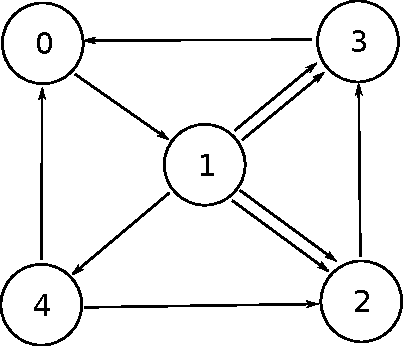
\includegraphics[scale=0.6]{figures/tiny_www.pdf}}
\end{center}

\pause
\bigskip

and a file \lstinline{tiny.txt} that encodes it
 
\begin{lstlisting}[language={}]
$ more tiny.txt
5
0 1
1 2 1 2
1 3 1 3
1 4
2 3
3 0
4 0 4 2
\end{lstlisting}
\end{frame}

\section{Transition Matrix}
\begin{frame}[fragile]
\pause

The transition matrix $P$ for a www with $N$ pages is an $N$-by-$N$ matrix such that the entry $P_{ij}$, ie, the entry in row $i$ and column $j$, is the probability that the random surfer moves to page $j$ when on page $i$

\pause
\bigskip

For example, a transition matrix for our tiny five-page web is
\[
P = \begin{bmatrix}
.02 & .92 & .02 & .02 & .02 \\
.02 & .02 & .38 & .38 & .20 \\
.02 & .02 & .02 & .92 & .02 \\
.92 & .02 & .02 & .02 & .02 \\
.47 & .02 & .47 & .02 & .02
\end{bmatrix}
\]
\end{frame}
\begin{frame}[fragile]
\pause

\begin{framed}
\tiny transition.py: Read links from standard input and write the corresponding transition matrix to standard output. First, process the input to count the outlinks from each page. Then apply the 90-10 rule to compute the transition matrix. Assume that there are no pages that have no outlinks in the input.
\end{framed}

\begin{lstlisting}[language=Python]
import stdarray
import stdio

n = stdio.readInt()
linkCounts = stdarray.create2D(n, n, 0)
outDegrees = stdarray.create1D(n, 0)
while not stdio.isEmpty():
    i = stdio.readInt()
    j = stdio.readInt()
    outDegrees[i] += 1
    linkCounts[i][j] += 1
stdio.writeln(str(n) + ' ' + str(n))
for i in range(n):
    for j in range(n):
        p = (.90 * linkCounts[i][j] / outDegrees[i]) + (.10 / n)
        stdio.writef('%8.5f', p)
    stdio.writeln()
\end{lstlisting}

\pause

\begin{lstlisting}[language={}]
$ python3 transition.py < tiny.txt
5 5
 0.02000 0.92000 0.02000 0.02000 0.02000
 0.02000 0.02000 0.38000 0.38000 0.20000
 0.02000 0.02000 0.02000 0.92000 0.02000
 0.92000 0.02000 0.02000 0.02000 0.02000
 0.47000 0.02000 0.47000 0.02000 0.02000
\end{lstlisting}
\end{frame}

\section{Simulating a Random Surfer}
\begin{frame}[fragile]
\pause

\begin{framed}
\tiny randomsurfer.py: Accept an integer $moves$ as a command-line argument. Read a transition matrix from standard input. Perform $moves$ moves as prescribed by the transition matrix, and write to standard output the relative frequency of hitting each page, ie, its page rank.
\end{framed}

\begin{minipage}{170pt}
\begin{lstlisting}[language=Python]
import random
import stdarray
import stdio
import sys

moves = int(sys.argv[1])
n = stdio.readInt()
stdio.readInt()
p = stdarray.create2D(n, n, 0.0)
for i in range(n):
    for j in range(n):
        p[i][j] = stdio.readFloat()
hits = stdarray.create1D(n, 0)
page = 0
for i in range(moves):
    r = random.random()
    total = 0.0
    for j in range(0, n):
        total += p[page][j]
        if r < total:
            page = j
            break
    hits[page] += 1
for v in hits:
    stdio.writef("%8.5f", 1.0 * v / moves)
stdio.writeln()
\end{lstlisting}
\end{minipage}
\begin{minipage}{130pt}
\visible<2->{
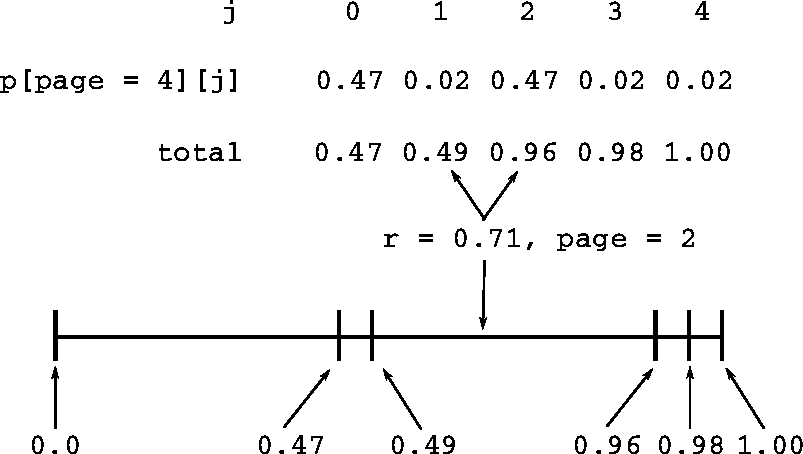
\includegraphics[scale=0.35]{figures/roulette.pdf}
}
\end{minipage}
\end{frame}

\begin{frame}[fragile]
\pause

\begin{lstlisting}[language={}]
$ python3 transition.py < tiny.txt | python3 randomsurfer.py 100
 0.26000 0.27000 0.18000 0.26000 0.03000
\end{lstlisting}

\pause

\begin{lstlisting}[language={}]
$ python3 transition.py < tiny.txt | python3 randomsurfer.py 10000
 0.27410 0.26500 0.14570 0.24890 0.06630
\end{lstlisting}

\pause

\begin{lstlisting}[language={}]
$ python3 transition.py < tiny.txt | python3 randomsurfer.py 10000000
 0.27308 0.26568 0.14616 0.24719 0.06789
\end{lstlisting}
\end{frame}

\section{Markov Chain}
\begin{frame}[fragile]
\pause

A Markov chain is a random process that describes behavior similar to the random surfer

\pause
\bigskip

An useful property of Markov chains is that of mixing, which states that the random surfer could start anywhere, since the probability that the surfer eventually winds up on any particular page is the same for all starting pages

\pause
\bigskip

Using the power method we can obtain the probability $P^2_{ij}$ that the random surfer will move from page $i$ to page $j$ in two moves by squaring the transition matrix $P$ $$P^2_{ij} = P_{i:} \cdot P_{:j}$$ 

\pause
\bigskip

For example, for our tiny web, we have
\begin{align*}
P^2_{ij} &= 
\begin{bmatrix}
.02 & .92 & .02 & .02 & .02 \\
.02 & .02 & .38 & .38 & .20 \\
.02 & .02 & .02 & .92 & .02 \\
.92 & .02 & .02 & .02 & .02 \\
.47 & .02 & .47 & .02 & .02
\end{bmatrix}
\cdot
\begin{bmatrix}
.02 & .92 & .02 & .02 & .02 \\
.02 & .02 & .38 & .38 & .20 \\
.02 & .02 & .02 & .92 & .02 \\
.92 & .02 & .02 & .02 & .02 \\
.47 & .02 & .47 & .02 & .02
\end{bmatrix} \\
& =
\begin{bmatrix}
.05 & .04 & .36 & .37 & .19 \\
.45 & .04 & .12 & .37 & .02 \\
.86 & .04 & .04 & .05 & .02 \\
.05 & .85 & .04 & .05 & .02 \\
.05 & .44 & .04 & .45 & .02
\end{bmatrix} 
\end{align*}

\end{frame}

\begin{frame}[fragile]
\pause

In general, the probability that the random surfer will move from page $i$ to page $j$ in $t$ moves is obtained by computing $P^t$ 

\pause
\bigskip 

Unfortunately, matrix-matrix multiplication is expensive

\pause
\bigskip

Fortunately, because of the mixing property, we can make do with relatively inexpensive vector-matrix multiplications

\pause
\bigskip

For example, with our tiny web, if we start with the vector 
\[
\begin{bmatrix}
1.0 & 0.0 & 0.0 & 0.0 & 0.0
\end{bmatrix}
\]
specifying that the random surfer starts on page 0, multiplying the vector by the transition matrix $P$ gives the vector 

\[
\begin{bmatrix}
1.0 & 0.0 & 0.0 & 0.0 & 0.0
\end{bmatrix}
\cdot
\begin{bmatrix}
.02 & .92 & .02 & .02 & .02 \\
.02 & .02 & .38 & .38 & .20 \\
.02 & .02 & .02 & .92 & .02 \\
.92 & .02 & .02 & .02 & .02 \\
.47 & .02 & .47 & .02 & .02
\end{bmatrix} = 
\begin{bmatrix}
.02 & .92 & .02 & .02 & .02
\end{bmatrix}
\]

specifying the probabilities that the surfer winds up on each of the pages after one step
\end{frame}

\begin{frame}[fragile]
\pause

Now, multiplying the above vector by the transition matrix $P$ again gives the vector
\[
\begin{bmatrix}
.02 & .92 & .02 & .02 & .02
\end{bmatrix}
\cdot
\begin{bmatrix}
.02 & .92 & .02 & .02 & .02 \\
.02 & .02 & .38 & .38 & .20 \\
.02 & .02 & .02 & .92 & .02 \\
.92 & .02 & .02 & .02 & .02 \\
.47 & .02 & .47 & .02 & .02
\end{bmatrix} =
\begin{bmatrix}
.05 & .04 & .36 & .37 & .19
\end{bmatrix}
\]
which contains the probabilities that the surfer winds up on each of the pages after two steps

\pause
\bigskip

The vector giving the probabilities that the random surfer is at each page after $t$ steps is the product of the corresponding vector for $t-1$ steps and the transition matrix $P$
\end{frame}

\begin{frame}[fragile]
\pause

\begin{framed}
\tiny markov.py: Accept integer $moves$ from the command-line, and read a transition matrix from standard input. Compute the probabilities that a
random surfer lands on each page (page ranks) after $moves$ matrix-vector multiplications, and write the page ranks to standard output.
\end{framed}

\begin{lstlisting}[language=Python]
import stdarray
import stdio
import sys

moves = int(sys.argv[1])
n = stdio.readInt()
stdio.readInt()
probs = stdarray.create2D(n, n, 0.0)
for i in range(n):
    for j in range(n):
        probs[i][j] = stdio.readFloat()
ranks = stdarray.create1D(n, 0.0)
ranks[0] = 1.0
for i in range(moves):
    newRanks = stdarray.create1D(n, 0.0)
    for j in range(n):
        for k in range(n):
            newRanks[j] += ranks[k] * probs[k][j]
    ranks = newRanks
for rank in ranks:
    stdio.writef("%8.5f", rank)
stdio.writeln()
\end{lstlisting}

\pause

\begin{lstlisting}[language={}]
$ python3 transition.py < tiny.txt | python3 markov.py 20
 0.27245 0.26515 0.14669 0.24764 0.06806
\end{lstlisting}

\pause

\begin{lstlisting}[language={}]
$ python3 transition.py < tiny.txt | python3 markov.py 40
 0.27303 0.26573 0.14618 0.24723 0.06783
\end{lstlisting}
\end{frame}
\end{document}
